%!TEX root = Report.tex
\chapter{Analysis Procedure}\label{sec:methodofattack}


\section{Imaging System}

\begin{figure}[H]
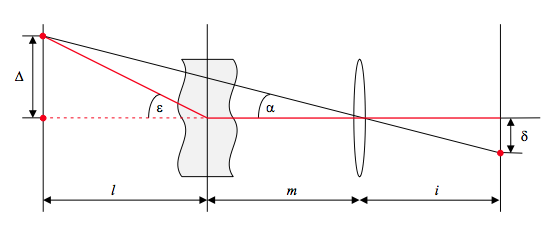
\includegraphics[width=1\textwidth]{pics/geometry}
\caption{Geometry Of The Optical Setup}
\label{pic:geometry}
\end{figure}


From the geometry of the optical setup shown in figure \ref{pic:geometry}, we can derive the following relations:
\\
\begin{equation}
\tan(\epsilon)=\frac{\Delta}{l}
\label{eq:geom1}
\end{equation}

\begin{equation}
o=l+m
\label{eq:geom2}
\end{equation}

\begin{equation}
\tan(\alpha)=\frac{\Delta}{o}=-\frac{\delta}{i}
\label{eq:geom3}
\end{equation}\\

The lens equation is as well given by:
\\
\begin{equation}
\frac{1}{o}+\frac{1}{i}=\frac{1}{f}
\label{eq:lenseq}
\end{equation}\\

Combining equations \ref{eq:geom1}, \ref{eq:geom2}, \ref{eq:geom3} and \ref{eq:lenseq} using the limit for large image imaging distances $o>>f$, we obtain equation \ref{eq:imdispl}:

\begin{equation}
\delta \approx \frac{f}{1+ \frac{m}{l}} \tan(\epsilon)
\label{eq:imdispl}
\end{equation}

which ist the image displacement on the sensor surface.
\\

For the cumulative deflection vector field, we use equation \ref{eq:intgradn} (with $l \rightarrow \infty$):
\\
\begin{equation}
\vec{\delta}(x,y)\approx -f \cdot \tan(\epsilon)=- \frac{f}{n_0}\int_{-\infty}^{+\infty} \mathrm \nabla n_1(x,y,z)\,\mathrm dz
\label{eq:intgradn}
\end{equation}


\section{Wedge calibration}

With MATLAB, we read in the images and crop an area in the middle of the wedge prism. These cropped images are then auto-correlated to the reference image and the positions of the correlation peaks are compared. Therefrom we obtain the deflection (=image shifts). In the following equation \ref{eq:deltawedge}, the deflection $\left| \delta^{1^\circ}_{pix}(l) \right|$ for the wedge prism is derived:\\

\begin{equation}
\left| \delta^{1^\circ}_{pix}(l) \right|=\kappa \frac{lf}o \tan({1^\circ}) \ [pixel]
\label{eq:deltawedge}
\end{equation}\\

Where $\kappa$ is the pixel size ($[\kappa]=\frac {pixels}{m}$), $l$  the distance from the object to the background image, $f$ the focal length of the camera and $o$ the distance between camera and background image.\\

For subsequent measurement we can use the scaling relation:\\

\begin{equation}
\frac{\tan(\vec{\epsilon})} {\tan(1^\circ)} = - \frac{\vec \delta_{pix}} {\left |\delta^{1^\circ}_{pix}(l) \right |}
\label{eq:scalrel}
\end{equation}\\

Where $\vec \epsilon$ is the deflection angle. \\


\section{Convection Cell}

A given MATLAB script 'SimplePIV' calculates the image shifts. The refractive index gradient can be calculated with Equation \ref{eq:gradn}, which is simplified with the scaling relation from Equation \ref{eq:scalrel}:
\begin{equation}
\vec\nabla n \approx \frac{n_0}{L} \tan(\vec{\epsilon})=-\frac{n_0}{L}\tan(1^\circ) \frac{\vec\delta_{pix}}{|\delta_{pix}^{1^\circ}(l)|}
\label{eq:gradn}
\end{equation}
where $L$ is the length of the test cell (10 mm).\\

The refractive index gradient from \ref{eq:gradn} can then be integrated (with boundary conditions) to obtain the refractive index. In our experiment, we can use a provided MATLAB file 'IntegrateDisplacements' for the integration. The boundary condition is a constant refractive index on the right hand side of the flow cell (side without electrical heating). We can't use the direct displacements calculated before and have to multiply it with a scaling factor $\phi=\sigma \cdot \gamma$ where $\sigma$ is the pixel scale factor ($\sigma=[\frac{m}{pixel}]$) and $\gamma$ the grid unit (i.e. the increment parameter in the 'SimplePIV' method with $\gamma=\frac{\text{pixel}}{\text{gridunit}}$).\\

Finally, the temperature field can then be calculated with Equation \ref{eq:nparafin}.
The MATLAB file can be seen in the Appendix.